\documentclass[english,11pt]{beamer}

\DeclareMathOperator{\Cov}{Cov}
\DeclareMathOperator{\Var}{Var}
\DeclareMathOperator{\E}{\mathbb{E}}
\DeclareMathOperator{\Proba}{\mathbb{P}}

\newcommand{\Covb}[2]{\ensuremath{\Cov\!\left[#1,#2\right]}}
\newcommand{\Eb}[1]{\ensuremath{\E\!\left[#1\right]}}
\newcommand{\Pb}[1]{\ensuremath{\Proba\!\left[#1\right]}}
\newcommand{\Varb}[1]{\ensuremath{\Var\!\left[#1\right]}}

% norm
\newcommand{\norm}[1]{\| #1 \|}

\newcommand{\indep}{\rotatebox[origin=c]{90}{$\models$}}





\usepackage{mathptmx,amsmath,amssymb,graphicx,bibentry,bbm,babel,ragged2e}

\makeatletter

\newcommand{\noun}[1]{\textsc{#1}}
\newcommand{\jitem}[1]{\item \begin{justify} #1 \end{justify} \vfill{}}
\newcommand{\sframe}[2]{\frame{\frametitle{#1} #2}}

\newenvironment{centercolumns}{\begin{columns}[c]}{\end{columns}}
%\newenvironment{jitem}{\begin{justify}\begin{itemize}}{\end{itemize}\end{justify}}

\usetheme{Warsaw}
\setbeamertemplate{footline}[text line]{}
\setbeamercolor{structure}{fg=purple!50!blue, bg=purple!50!blue}

\setbeamersize{text margin left=15pt,text margin right=15pt}

\setbeamercovered{transparent}


\@ifundefined{showcaptionsetup}{}{%
 \PassOptionsToPackage{caption=false}{subfig}}
\usepackage{subfig}

\usepackage[utf8]{inputenc}
\usepackage[T1]{fontenc}

\usepackage{multirow}


\makeatother

\begin{document}





\title{Validation of geosimulation models: a systematic review}

\author{J.~Raimbault$^{1,2,3,4,\ast}$\\
\texttt{$\ast$ juste.raimbault@ign.fr}
}


\institute{$^{1}$ LASTIG, IGN-ENSG\\
$^{2}$CASA, UCL\\
$^{3}$UPS CNRS 3611 ISC-PIF\\
$^{4}$UMR CNRS 8504 G{\'e}ographie-cit{\'e}s
}


\date{ECTQG 2023\\\smallskip
Session Theoretical Geography 2\\\smallskip
September 15th 2023
}

\frame{\maketitle}




%Keywords: Geosimulation models, Validation, Systematic review
%Geosimulation models are a widely used tool in theoretical and quantitative geography, and deemed powerful for various reasons including their ability to capture spatial complexity, a heterogeneity of agent and processes, or multiple scales. One downside of their subsequent high parameter space or strong stochasticity, of the need to explicitly simulate them to understand their behaviour, and of their flexibility, is that their validation is less systematic than for their statistical, machine learning or analytical counterparts, for which robust criteria are available. Furthermore, the concept of model validation or evaluation seems to be contextual to the disciplinary environment in which the model is developed and used.
%This contribution proposes a systematic review of how the concept of validation is defined and used for geosimulation models. Using the data collection tools provided by Raimbault (2019), we construct a corpus by querying google scholar. We follow the PRISMA guidelines for systematic reviews, and screen titles of a first corpus of around 1000 papers, and then abstracts, to obtain an exploitable corpus of around 200 papers with an explicit reference to validation methods for a geosimulation model. We extract from these papers characteristics including the method used, the type of model, and the discipline. We finally obtain a typology of validation methods in a broad sense, ranging from sensitivity analysis to uncertainty quantification or qualitative behavior regarding stylised facts. Methods used are correlated to the discipline and the type of model.
%We then reconstruct the backward citation network from our initial corpus at depth two using the same data collection tool, to provide a more general literature mapping and an overview the diversity of disciplines using spatial simulation models, which include for example ecology, social and urban simulation or geosciences. The plurality of approaches confirms the need for a flexible concept of validation and the diversity of associated methods.




\sframe{When is a simulation model ``validated''?}{

% illustration: LUTI applied vs overexplored opinion model more difficult to apply


\begin{center}
	\includegraphics[width=0.55\textwidth]{../../../../../Teaching/2018-OACMO/CM/figures/LUTI_irpud.png}
	%
	\hspace{0.5cm}
	%\externalfigure[https://www.jasss.org/22/4/10/Figure5.PNG]
	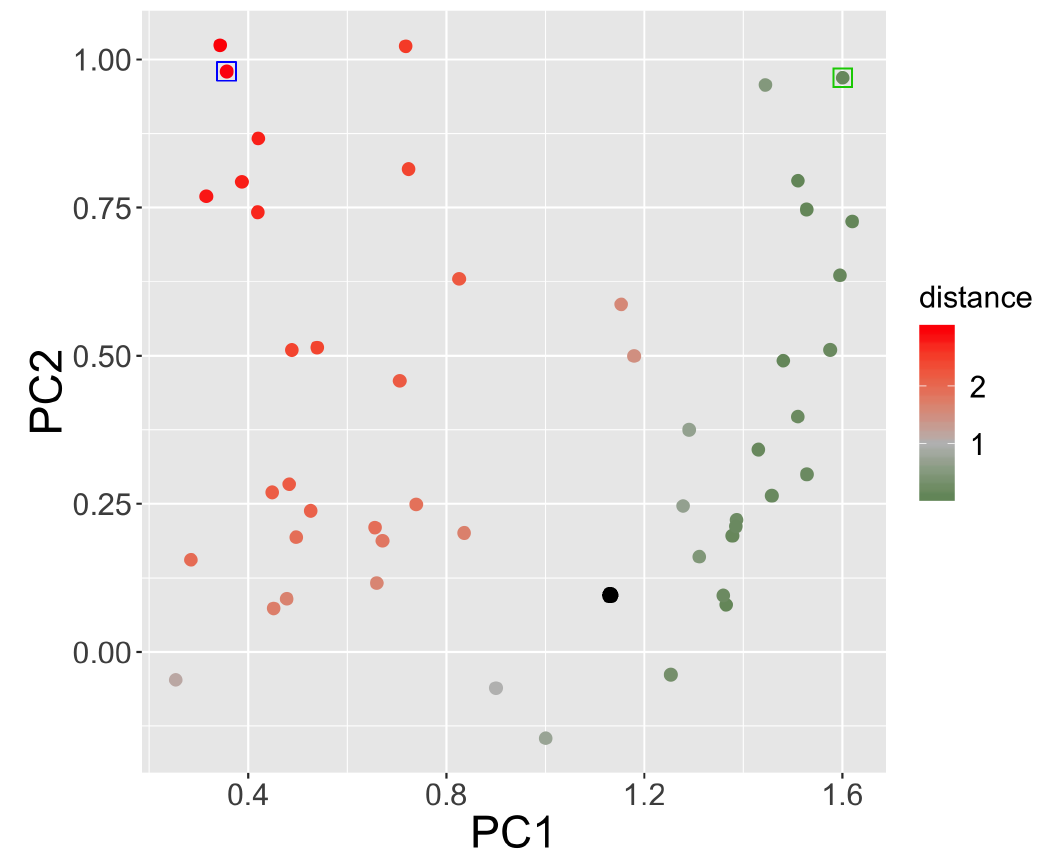
\includegraphics[width=0.35\textwidth]{figures/Figure5.png}
\end{center}

(Left) Operational large microsimulation model for land-use transport interactions \cite{wegener2011irpud}; (Right) Systematic exploration and comparison of phase diagrams across meta-parameter space for a toy model (sugarscape) \cite{raimbault2019space}
 


}

\sframe{Specificities for simulation models}{

% Geosimulation models are a widely used tool in theoretical and quantitative geography, and deemed powerful for various reasons including their ability to capture spatial complexity, a heterogeneity of agent and processes, or multiple scales. One downside of their subsequent high parameter space or strong stochasticity, of the need to explicitly simulate them to understand their behaviour, and of their flexibility, is that their validation is less systematic than for their statistical, machine learning or analytical counterparts, for which robust criteria are available.

\textbf{Advantages} of geosimulation models: spatial complexity, heterogeneity of agents and processes, multiple scales, come at the cost of a more difficult validation:

\bigskip

\begin{itemize}
	\item High-dimensional parameter space and output space
	\item Strongly non-linear, non-ergodic, non-stationary dynamics
	\item Stronger role of stochasticity
	\item Need to be fully simulated (weak emergence)	
\end{itemize}



}


\sframe{Disciplinary definitions of validation}{

% Furthermore, the concept of model validation or evaluation seems to be contextual to the disciplinary environment in which the model is developed and used.

\textbf{Definition} of ``model validation'' strongly depends on disciplines, methods, type of models, for example:

\bigskip

\begin{itemize}
	\item metrics linked to prediction performance for machine learning
	\item resembling patterns in Pattern Oriented Modelling \cite{grimm2005pattern}
	\item ``face validity'' in agent-based models
	\item advanced validation toolset with the OpenMOLE platform \cite{reuillon2013openmole}
	\item stakeholders' feedback in participatory approaches
	\item \ldots
\end{itemize}



}



\sframe{A proposal based on model functions}{

% recall presentation CCS2019 satellite: validation tightly linked with model function in the sense of Varenne

Proposal for a typology of model validation techniques and standards by \cite{raimbault2020validation}, based on \cite{varenne2018theories}'s typology of model functions and modeller purpose \cite{giere2019scientific}:

\medskip

\begin{itemize}
	\item \textbf{Perception and observation}: how much information is extracted
	\item \textbf{Description}: how much information is contained within
	\item \textbf{Prediction}: predictive power (quantitative indicators or qualitative behavior)
	\item \textbf{Explication and comprehension}: how much of the causal structure of the system is grasped
	\item \textbf{Theory construction}: how does the model contributes to the theory, to coupling of its components (e.g. medium for interdisciplinarity)
	\item \textbf{Communication}: how much information is conveyed and to which agents
	\item \textbf{Decision-making}: how are decision supported, which benefits and for what dimension (societal, environmental, etc.)?
\end{itemize}


}


\sframe{Contribution}{

% This contribution proposes a systematic review of how the concept of validation is defined and used for geosimulation models.

$\rightarrow$ geosimulation/spatial simulation models are used in a wide range of disciplines

\bigskip

$\rightarrow$ what are effective ``validation'' practices of these diverse scientific communities?

\bigskip
\bigskip

\textbf{This contribution: } \textit{propose a Systematic Review of the concept of validation for geosimulation models.}


}


\sframe{Systematic review}{

% Using the data collection tools provided by Raimbault (2019), we construct a corpus by querying google scholar. We follow the PRISMA guidelines for systematic reviews, and screen titles of a first corpus of around 1000 papers, and then abstracts, to obtain an exploitable corpus of around 200 papers with an explicit reference to validation methods for a geosimulation model.
% We extract from these papers characteristics including the method used, the type of model, and the discipline.


$\rightarrow$ using data collection tools developed by \cite{raimbault2019exploration}, construct a paper corpus through a keyword request to google scholar

\bigskip

$\rightarrow$ systematic screening of paper titles (and abstracts/full texts if needed) to keep relevant papers

\bigskip

$\rightarrow$ extraction of method and models characteristics: discipline (from journal/affiliation), type of method (ad hoc typology), type of model (idem), generic methodological contibution

\bigskip

$\rightarrow$ ``meta-analysis'' of corpus characteristics

}


\sframe{PRISMA systematic review description}{

% list relevant reporting items with detailed description

% -> remarks to be kept for discussion: "soft SR", intermediate, fuzzy concepts, defs etc: in general SR in social sci? boundaries and purpose of SRs?

Relevant PRISMA reporting points:
% http://www.prisma-statement.org/PRISMAStatement/Checklist % not needed

\footnotesize

\begin{itemize}
	\item[5] - \textbf{Eligibility criteria: } explicit reference to ``validation'' (and synonyms) in the title/abstract
	\item[6] - \textbf{Information sources: } google scholar, accessed through the \texttt{BiblioData} API \cite{raimbault2019exploration}
	\item[7] - \textbf{Search strategy: } direct query: ("spatial simulation"OR"geosimulation")AND("validation"OR"calibration"OR"\\
	sensitivity analysis"OR"exploration"OR"evaluation"OR"\\
	assessment")
	\item[8] - \textbf{Selection process: } manual screening of titles (/abstracts/full text) by one expert
	\item[9] - \textbf{Data collection process: } manual extraction by one expert during screening (if included)
	\item[10] - \textbf{Data items: } discipline (journal/affiliation), method (ad hoc typology), type of model, methodological work
	\item[13] - \textbf{Synthesis methods: } statistical analysis of categorical variables
\end{itemize}




}


\sframe{Systematic review flowchart}{

% QUERY:
% ("spatial simulation"OR"geosimulation")AND("validation"OR"calibration"OR"sensitivity analysis"OR"exploration"OR"evaluation"OR"assessment")
% according to scholar: ~ 1840 results
% query result: 852 papers
% title screening: explicit mention of validation/calibration/etc. in title ["meta" in some sense]
% extract: discipline, method, type of model, generic methodo? : title, abstract/full text screening if needed ; spatial-specific method? ~ difficult to evaluate
% ! bias to be overcome using ML? or more time for systematic screening: DECLARATIVE validation, in title: strong influence of disciplinary practices (or other context parameters)
% note; purely technical contribs have been removed (parallelisation, HPC) - they are an other aspect of validation?
% note: corpus not weighted (// reviews in luti for example)
%  - duplicates? ~ -> noise
%. => analysis corpus 132 refs (not 200: more cleaning ~)

\centering

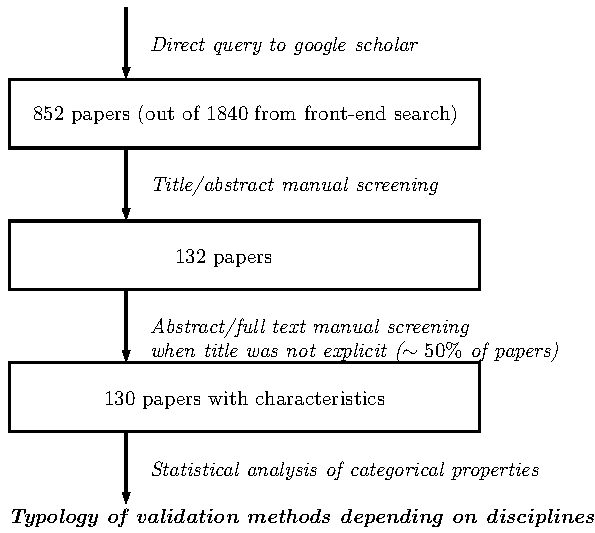
\includegraphics[width=0.8\textwidth]{figures/sr.pdf}



}




\sframe{Results: disciplines}{

%We finally obtain a typology of validation methods in a broad sense, ranging from sensitivity analysis to uncertainty quantification or qualitative behavior regarding stylised facts. 

\textbf{Disciplines (on 130 papers):} ecology (28), geosimulation (26), land-use change (18), environmental science (15), urban science (11), hydrology (11), computer science (8), sustainability (6), climate science (4), archeology (1), biology (1), social science (1)

\bigskip

$\rightarrow$ sampling rate of the corpus unknown (need to cross with other databases), but proportions seem reasonable


\bigskip

$\rightarrow$ some ``hard'' disciplines missing or under-represented (physics, climate science): validation is intrinsic to their modelling enterprise and not explicitly mentioned?

\bigskip

$\rightarrow$ validation methodologies from ecology to social sciences? (cf ABM and POM)


}

\sframe{Results: typology of validation methods}{

\textbf{Ad hoc typology of validation methods: }

\begin{columns}
	\begin{column}{0.49\textwidth}
		\begin{itemize}
	   \item prediction (24)
	   \item SA (19)
	   \item uncertainty (18)
	   \item multiple (13)
	   \item benchmark (12)
	   \item calibration (11)
	   \item optimisation (9)
\end{itemize}
	\end{column}
	\begin{column}{0.49\textwidth}
		\begin{itemize}
	   \item visualisation (8)
	   \item POM (6)
	   \item participatory (4)
	   \item exploration (3)
	   \item mixed (2)
	   \item surrogate (1)
\end{itemize}
	\end{column}
\end{columns}

\bigskip

$\rightarrow$ A relatively exhaustive list of method types?

\bigskip

$\rightarrow$ proportions not representative: implicit validation in many disciplines and methods



}


\sframe{Results: disciplinary context}{

% Methods used are correlated to the discipline and the type of model.


% + 1 other slide results: ? facts to note, generic methodo?

% contingency table! (statistical test TBD? maybe not worth it given bias/missing data?)

\resizebox{\linewidth}{!}{
\begin{tabular}{l|ccccccccc|}
& benchmark & calibration & multiple & optimisation & POM & prediction & SA &  uncertainty & visualisation \\\hline
computer science & 0  & 3   &  3   & 1   &  0    & 0   & 0   &  0 & 1 \\
ecology   & 3  &  2 & 2  & 3   &  2  & 6  &  4 & 4 & 0 \\
environmental science & 2 & 2 & 0 & 0 & 0 & 0 & 2  & 8 & 1\\
geosimulation   & 0    & 2   & 2   &  0   &  0    &  4   & 5   & 5 & 3 \\
hydrology   & 1    & 1   & 0   &  2   &  0   & 4   & 2    & 0 & 0 \\
land-use change   & 3   &  0    &  3    & 1   &  3   & 7   & 1   & 0 & 0 \\
sustainability   &  0   & 1    & 0   & 1   & 0   & 0   & 0    &  0 & 3 \\
urban science   &  0    &  0   & 3   & 1    & 1    & 1   & 4    & 0 & 0 \\
\end{tabular}
}

}

% ~ - no time
%\sframe{Results: methodological contributions}{
%}



\sframe{Broader literature mapping: citation network}{

% We then reconstruct the backward citation network from our initial corpus at depth two using the same data collection tool, to provide a more general literature mapping and an overview the diversity of disciplines using spatial simulation models, which include for example ecology, social and urban simulation or geosciences.



}

	



\sframe{Discussion: SR/MA methodology}{

% cite MA networksterrit ! -> same lessons ~, more difficult here as methodo? (depends on knowledge domains?)

% The plurality of approaches confirms the need for a flexible concept of validation and the diversity of associated methods.

% - discussion on SR methodo: more to be done - ML? model decomposition approach?

% - need for a more emdogenous typology, as in model decomposition (Q: how initial categs done?): based on types? categ th?

% - weight and duplicate reviews?

% - thn for each class of the typology, list metrics?

% discuss represntativite du corpus: tres difficile!

% ENJEU principal des SR/MA en interdisciplinarite: find endogenous equivalences between defs, concepts, methods: ? (same Q as ``bridges'' - cf soc nw/physics, etc.) -> method to be invented!

% Comment OML integre la plupart des methods, companion model exlporation, pub exmod a la fin!

% bias: ex explo/DOE pas explicitement mentionne mais naturel dans une mesure minimale
% idem "internal/statistical validation" done but not mentionned

% IDEA: first endoge disc/map, then specific SR within each, then endog contruction of equivalences?


% \textbf{Main results:}


\justify

$\rightarrow$ 
			
\bigskip
				
$\rightarrow$ 

\bigskip

% separated or not?
%\textbf{Conclusion: } 

}


\sframe{Discussion: towards interdisciplinary validation standards?}{

% ! role of reflexivity and quantep/lit mapping: cit cybnws! ; knowledge domains?

}









%%%%%%%%%%%%%%%%%%%%%
\begin{frame}[allowframebreaks]
\frametitle{References}
\bibliographystyle{apalike}
\bibliography{biblio}
\end{frame}
%%%%%%%%%%%%%%%%%%%%%%%%%%%%




\end{document}









